In the category \(\mathbf{Graph}\) pushouts always exist, and their construction is straightforward when dealing with monomorphisms (injective graph homomorphisms). 
% Let $\uplus$ denote the disjoint union operation. For two sets \(A\) and \(B\), their disjoint union \(A \uplus B\) is defined as the set of ordered pairs \( (x, i) \) where \( x \in A \) if \( i = 1 \) and \( x \in B \) if \( i = 2 \). Formally, we have:
% $
% A \uplus B = \{ (x, 1) : x \in A \} \cup \{ (x, 2) : x \in B \}.
% $ 
We denote $X\uplus Y$ the union of two disjoint sets. By possibly renaming nodes, a span of injective graph homomorphisms can be represented as
$
A \uplus B' \overset{\alpha}{\leftarrowtail} A \overset{\beta}{\rightarrowtail} A \uplus C'
$
where $A,B',C'$ are disjoint sets and $\alpha$ and $\beta$ are inclusion function. A pushout of this span is then given by
$
A \uplus B'  \overset{\beta'}{\rightarrowtail} A \uplus B' \uplus C'   \overset{\alpha'}{\leftarrowtail} A \uplus C'
$ where $\alpha'$ and $\beta'$ are inclusion function. This situation can be depicted by the diagram in \autoref{fig:po_decomp}
\begin{figure}[htbp] 
    \begin{center}
    \resizebox{0.45\textwidth}{!}{
        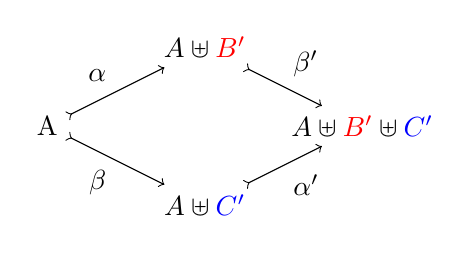
\begin{tikzpicture}
                    \node (i) at (0,0) {A};
                    \node (r) at (2,1) {$A \uplus \textcolor{red}{B'}$};
                    \node (c) at (2,-1) {$A \uplus \textcolor{blue}{C'}$};
                    \node (h) at (4,0) {$A \uplus \textcolor{red}{B'} \uplus \textcolor{blue}{C'}$};
                    \draw[>->]  (i) -- (r) node [midway, above left] {$\alpha$};
                    \draw[>->] (c) -- (h) node [midway, below right] {$\alpha'$};
                    \draw[>->] (r) -- (h) node[midway, above right] {$\beta'$};
                    \draw[>->] (i) -- (c) node[midway, below left] {$\beta$};
        \end{tikzpicture}
    }
    \end{center}
    
    \caption{Construction of the pushout of a span of monomorphisms in \(\mathbf{Graph}\)}
    \label{fig:po_decomp}
\end{figure}
where \(B'\) and \(C'\) are colored to make evident this decomposition in a concrete example within \textbf{Graph} in \autoref{ex:po_in_graph}, where nodes and arrows are colored accordingly.
